\chapter{OVERVIEW OF THE RNA.BGSU.EDU DATA PIPELINE, DATABASE AND SUPPORTED
ON-LINE RESOURCES}

In this chapter I will discuss the \href{http://rna.bgsu.edu}{RNA.BGSU.EDU}
pipeline and database. The aim is provide the reader with an overview of the
pipeline and familiarity with concepts and design. This chapter will first
provide a context for my work on the pipeline by discussing the goals, rationale
for this work and the principles defining the design of the pipeline and
database. This will then discuss the scientific value of our pipeline followed
by the design and how it allows us to achieve the principles. Finally we will
provide an overview of the implementation. 

\section{Goals for the BGSU RNA pipeline}

One of the major grant activities in our lab is the development, maintenance and
extension of our data pipeline and database that imports data from new
RNA-containing structure files as they appear in PDB on a weekly basis. The
pipeline is a python and Matlab application that annotates all pairwise
nucleotide interactions, groups structurally similar RNA molecules into
equivalence sets, identifies high quality representative sets of RNA structures
and extracts and clusters RNA 3D motifs and stores all these derived data in a
locally maintained MySQL database.

We have developed these tools to achieve the aims of NIH founded work carried
out in collaboration with with Dr. John Westbrook and Dr. Helen Berman at the
Nucleic Acids Database (NDB). This is the sixth year of the collaboration, which
began in 2010. The aims of the grant are:

\begin{enumerate}
        \item Deepen our understanding of RNA 3D structure by extracting and
                organizing 3D motifs

        \item Improve our understanding of the structure variation of RNA
                molecules and RNA complexes by examining and comparing 3D
                structures assigned to the same sequence/structure "equivalence"
                class.

        \item Accelerate the study of the correspondence between RNA 3D
                structure and RNA sequence

        \item Provide annotations for RNA-protein interactions

        \item Develop new and extended tools for delivery, search and
                visualization of the RNA sequence and structure annotations
                described in Aims 1-4 and make them available in the NDB.
\end{enumerate}

As a part of the grant we provide annotations to NDB on a weekly basis. These
data include our nonredundant sets and associated equivalence sets, nucleotide
interaction annotations, as well as motif clusterings. In the near future we
will add RNA-protein interactions.

The data computed in our pipeline are used to support research resources. We
provide the RNA community with the BGSU RNA site, the RNA 3D motif library,
JAR3D, WebFR3D, R3DAlign, and R3D-2-MSA. As these resources require access to
up-to-date RNA structures, it is essential that the database and pipeline always
produce all the required data.

Secondly, it is essential that the pipeline be easy to maintain, extend and
improve by successive groups of graduate students and research associates. After
the departure of Anton Petrov and during most of my Ph.D. work it has been my
responsibility to maintain and update the pipeline and database. During the time
I was charged with these responsibilities major improvements were made to take
advantage of new mmCIF formats from PDB. The following projects are underway
that will extend the pipeline's capabilities: 
\begin{enumerate*}
        \item Poorna Roy is writing code to annotate nucleotide-amino acid
                interactions, 
        \item Maryam Husseieni is writing code to annotate and extract
                multi-helix functions and cluster them for the RNA 3D Motif
                Atlas, 
        \item Once finalized these results will be written into the database 
        \item We continue on an ongoing basis to improve base-pair annotation
                (Dr. Craig Zirbel), loop extraction (my work) and motif
                clustering.
\end{enumerate*} 
As soon as these new results and functions are tested and validated these
improvements will be integrated into the pipeline's weekly update functions.

Thus the operations goals for our database and pipeline are:
\begin{enumerate}
        \item The pipeline must store only correct data in the database
        \item The pipeline must run reliable each week to maintain current data
        \item The pipeline must be ease to maintain, update and improve
\end{enumerate}

In the next sections I will discuss how the changes I have made to the previous
version help us achieve these goals.

\section{Comparison of the current BGSU RNA pipeline to other resources}

We have evaluated other software options and found them unsuitable for our
current aims. The main resource we considered was the previous implementation by
Dr. Anton Petrov \cite{Petrov2012}. The implementation was a part of his dissertation research.
Much of the previous pipeline was not suitable for our current requirements.

First, the previous version did not work with mmCIF data. In December 2014, the
protein databank (PDB) transitioned from the outdated fixed columnar width  PDB
format to a new mmCIF format for all 3D structure data.

Second, the previous version of the database and pipeline did not work to ensure
the validity of data. Consequently, I discoverd that our database contained
"orphan data". Orphan data is data that is missing related information. For
example, there were structures which had been placed into an NR group, but we
had no information on the resolution. In addition, a careful reading of the code
showed it was possible for the pipeline to write incomplete data. Incomplete
data is when we do not write all annotations for a structure. For example, if
there are 100 annotated base pairs, writing 99 of them would constituent writing
incomplete data. My rewrite was aimed at fixing these issues as well as
usability of the pipeline.

Finally, the previous version did not centralize the core logic of the pipeline
in a module making the pipeline harder to maintain. To explain, all parts of the
pipeline have the same core logic as detailed in a later section. Each part of
the pipeline that computes data is referred to as a ``stage''. The stage is
primarily responsible for computing data, while the core manages ensuring that
the overall pipeline behaves correctly.

A good example of centralizing logic, is the logic for rolling back failed
imports and checking if data has been computed. The previous version had not
centralized this logic so adding new computations required the programmer to add
logic to ensure that these actions happened correctly. In addition, requests to
remote resources were not always retried leading to some requests being more
fragile than others.

Another potential option was to use is the
\href{https://github.com/pharmbio/sciluigi}{sciluigi} which is built off the
luigi package provided by Spotify. Sciluigi package contains a framework for
building pipelines and is being adopted by the bioinformatic community. I have
chosen not to use sciluigi because it was released after I had already written a
large portion of the pipeline. While sciluigi is a well designed framework it
does not offer a compelling reason to rewrite large portions of our existing
framework. Had it existed prior to my start I would have likely used it.

\section{Design requirements for the BGSU RNA pipeline and database}

In more detail, to support the research goals, our pipeline must fulfill the
following requirements.

\begin{enumerate}
        \item The pipeline must always keep the database in a valid state.
        \item The pipeline must operate efficiently and avoid recomputing data unnecessarily
        \item The pipeline should facilitate user control when manual operation is required.
        \item The pipeline must be as reliable as possible.
        \item The pipeline must be designed so additions will respect all constraints.
\end{enumerate}

We will discuss each requirement and the rationale behind each one.

\subsection{Maintaining validity of data}

For a database to remain valid, two properties must be maintained. First, the
database must be complete. This means that the database should not be left in a
state with any partial data for any structure. For example, the database should
not have partial base pair annotations for a given structure: it should have all
or none. This requirement must be respected because our data supports several
sources: equivalence classes of similar structures and the representatives sets
they support and the annotations we provided to NDB
\cite{CoimbatoreNarayanan2014}, also the R3D-2-MSA \cite{Cannone2015}, JAR3D
\cite{Roll2016}, WebFR3D \cite{Petrov2011a}, and R3DAlign \cite{Rahrig2013}
sites all rely on data produced by pipeline in the database.

\subsection{Ensuring the validity of the database}

The second property of a valid database is that it is consistent. Consistency is
best explained through an example. Keeping the database consistent means
preventing situations from arising where we annotate a base pair involving RNA
nucleotide residues that we have not yet created and stored in the database. In
database terms, this requirement is referred to as preventing "orphan data".
Whenever data are inconsistent any analysis or display of the stored data will
fail, for lack of referenent.

By striving to keep the database in a valid and consistent state, we ensure that
the database is always usable for analysis and display on webpages, even when
the pipeline fails to update with new data. Without this it would make our other
tools, such as JAR3D and RNA 3D Hub, unstable. Providing these resources in an
ongoing and stable manner is a major grant activity in the lab, which is why
this is the most important design consideration of the pipeline.

Preventing the writing of incomplete or orphan data is also essential to
avoiding or minimizing the unnecessary recomputation of data. As we learned
during the transition of CIF format files, which required the computation of
most annotations, recomping all data for each each run of the pipeline would
take several weeks. This is too slow and completely unnecessary for our planned
weekly update runs of the pipeline. Thus the pipeline is designed to only
compute data for new structures or manually specified structures that need to be
recomputed for some particular reason, at the manager's discretion.

\subsection{Controlling the pipeline}

The next priority, ease of controlling which stages and structures to run during
manual operation, is intended to facilitate error correction. Work with previous
version of the pipeline showed that extensive manual work was always needed to
rerun the correct stages with the correct data. This manual work was
error-prone, and frequently produced even more problems that need correction. By
automating the repetitive manual work, I succeeded in making it easier to
recover from errors.

\subsection{Pipeline Reliability}

The fourth consideration is that the pipeline must be as reliable as possible.
Reliability means that the pipeline will compute as much data as possible
despite errors. Errors in programs are inevitable and must be anticipated in the
design of the pipeline. Even if all parts of the pipeline are written correctly
it can still fail because of anomalous events generated by external resources.
For example, the pipeline has failed when:  PDB provided incomplete data or when
the network experienced instability during few fractions of a second required to
complete a web request. These and other issues that I have encountered during
the years I was responsible for pipeline operation, convinced me of the high
priority of making the pipeline as robust as possible.

The final consideration is ease of adding new "stages" to provide new
functionality as this will carried out on an ongoing basis by current and new
students involved in the project. They should be able to make changes without
having to know all the details of how the pipeline works, confident that they do
not have to deal with ensuring the validity of the database and the stability of
the pipeline in order to make improvements and additions of new functionality.

\section{Implementation of the BGSU RNA data pipeline}

In this section I discuss the improvements to the pipeline that enable it to
fulfill the design requirements outlined above. These improvements required
coordinated changes to occur both in the pipeline application and the database.
Each requirement in turn.

\subsection{Ensuring data validity}

To maintain validity of data in a database, it is essential to add constraints
to the database. Constraints are requirements on one or more columns that ensure
certain criteria must be met before adding or modifying data in that column. The
constraints I have added include uniqueness constraints and foreign key
constraints as appropriate. Constraints were added to  nearly every table in the
database. These constraints could not be added prior to these improvements
because the database was not configured to allow them.

A uniqueness constraint ensures that no two rows in the same table may have the
same data values in any column. Uniqueness constraints may span more than one
column. For example, I have added a uniqueness constraint on the ``pdb\_id'' and
``chain\_name'' column in the ``chain\_info" table. This table stores information
about all chains and by placing the uniqueness constraint on these two columns I
ensure that there can be no two chains in the same structure with the same
combination of PDB id and chain name. This constraint reflects the logical
structure of the data. By adding these constraints, I ensure that the data in
the database is logically correct as regarding chains.

The second type of constraint I introduced is the consistent implementation of
foreign keys wherever required to allow the many tables in our database to work
together properly. These ensure that entries in one column of one table exist in
another column of another table. These safeguard data completeness. The use of
foreign keys allows the expression of the requirement of ``interactions must be
built from known residues'. To describe a specific example, we have a table
called ``unit\_info'' which contains data for all residues, RNA, DNA, protein,
ligands, etc, known in the database. In the unit\_info table there is a
``unit\_id'' column that provides a unique identifier for all units (i.e.
residues, whether RNA, DNA or protein). The ``unit\_pairs\_interactions'' table
contains all pairwise interactions between RNA residues, such as base pair and
base stacking interactions. It contains a ``unit\_id\_1'' and ``unit\_id\_2'' column
which specify the first and second units forming the interaction. For an
interaction represented by a row in the unit\_pairs\_interactions table to be
valid, the entries in the ``unit\_id\_1'' and ``unit\_id\_2'' must exist  in the
``unit\_id'' column of the ``unit\_info'' table. I have enforced this logical
requirement by declaring that ``unit\_id\_1'' and ``unit\_id\_2'' are foreign keys
link to ``unit\_id'' in the unit\_info table.

At the level of the pipeline application, I ensure data validity by implementing
procedures to automatically rollback failed imports. Because we have foreign key
and uniqueness constraints, it is possible to attempt to write data that will be
rejected. For example, if the pipeline attempts to write an interaction between
units that do not exist, the database will reject the data because of the
foreign key constraints. I rewrote the pipeline so that in the event of such an
error during a data entry operation, all interactions that were written for that
structure will be deleted. This prevents the writing of partial data for any
single structure, ensuring the database remains complete, ie ensuring the
absence of partial data.

\subsection{Minimizing the number of computations}

If the pipeline were to recompute all data on every update a single run would
take at least several weeks to complete with currently available resources.
Given that we are committed to provide weekly updates to NDB, this is
unacceptable. However, the capability to easily force data to be recomputed is
also crucial. For example, we update our classification of pairing interactions
from time to time. When this is done, we must be able to easily update the
entire database with the new pairing annotations. I have implemented the
capability to make such updates by simply telling the pipeline to delete the old
data and recompute the new data.

I have changed the pipeline execution to first check whether data have already
been computed for each input and only computing data when none are present, or
when the user explicitly requests the pipeline to select recompute selected
data. Now as currently configured all parts of the pipeline go through the steps
shown in Figure~\ref{fig:stage-flow}. With this logic I can ensure that only the
required data are computed. The previous version of the pipeline had a similar
capability however my additions make it more comprehensive, as well as, ensuring
that old data are always deleted prior to recomputing existing data. In the
previous version it was not required that all parts have consistent behavior in
the face of existing data. I have centralized the logic for recomputing and
deleting old data.

\begin{figure}
  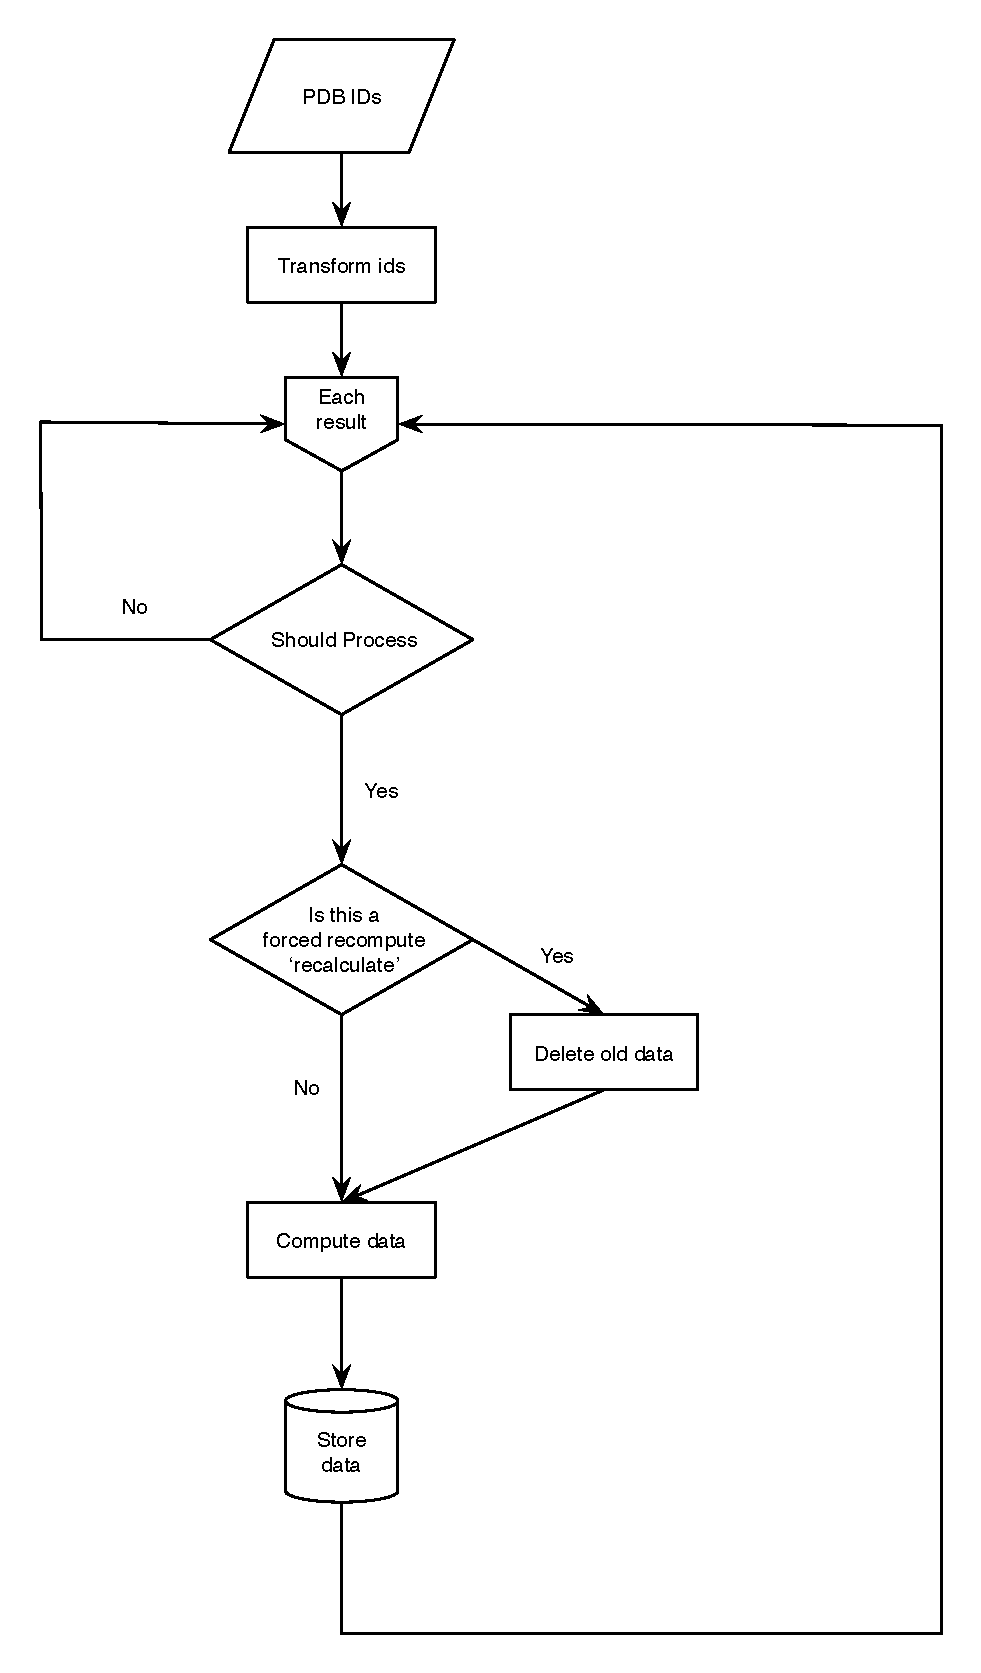
\includegraphics[height=8in]{chapter-2/figs/stage-flow}
\caption{Figure summarizing the logical flow for each stage. This figure shows
the general scheme of all stages.}
\label{fig:stage-flow}
\end{figure}

This requirement ensures efficient execution times of our pipeline. Without it
our weekly, or even monthly update schedule could not be maintained. However, in
order to correctly skip recomputing old data, the database must always be
complete. Should the pipeline begin to save incomplete data, it will never
attempt to recompute and fill in missing data. For this reason, it is essential
that the database always remain complete.

\subsection{Providing control over the data computed}

The day-to-day goal of the pipeline is to run weekly updates using all available
structures. In this case the intent is to compute all annotations for all
structures. However, it is often useful and sometimes necessary to run specific
annotations on specific structures. For example, when testing a new set of
annotations it is desirable to select a few test structures on which to run only
the new annotations, and then examine the results.

To make this possible, I have restructured the pipeline to provide a single
unified point of entry that takes as input the name of the part to run and the
particular structures to analyze, or an option to include all available
structures. In the previous version of the pipeline there were several possible
entry points. The primary entry point was the ``update'' component. This part
would run everything required for a weekly update in the correct order. The
other entry points were specific to individual components such as loading
interactions. This was an issue because parts of the pipeline have dependencies
upon each other. For example, to compute the pairwise interactions, the
structure must first be downloaded. Previously, these dependencies were implicit
in the design of the update component and were not stated explicitly, leading to
potential confusion.

These dependencies are now encoded into the pipeline using a dependency graph as
shown in Figure~\ref{fig:stage-deps}. This graph can be sorted using a topological
sort to produce a linear ordering. I have implemented this logic as part of the
``dispatcher'' which determines which modules to run and in which order to run
them in for a given application.


\begin{figure}
  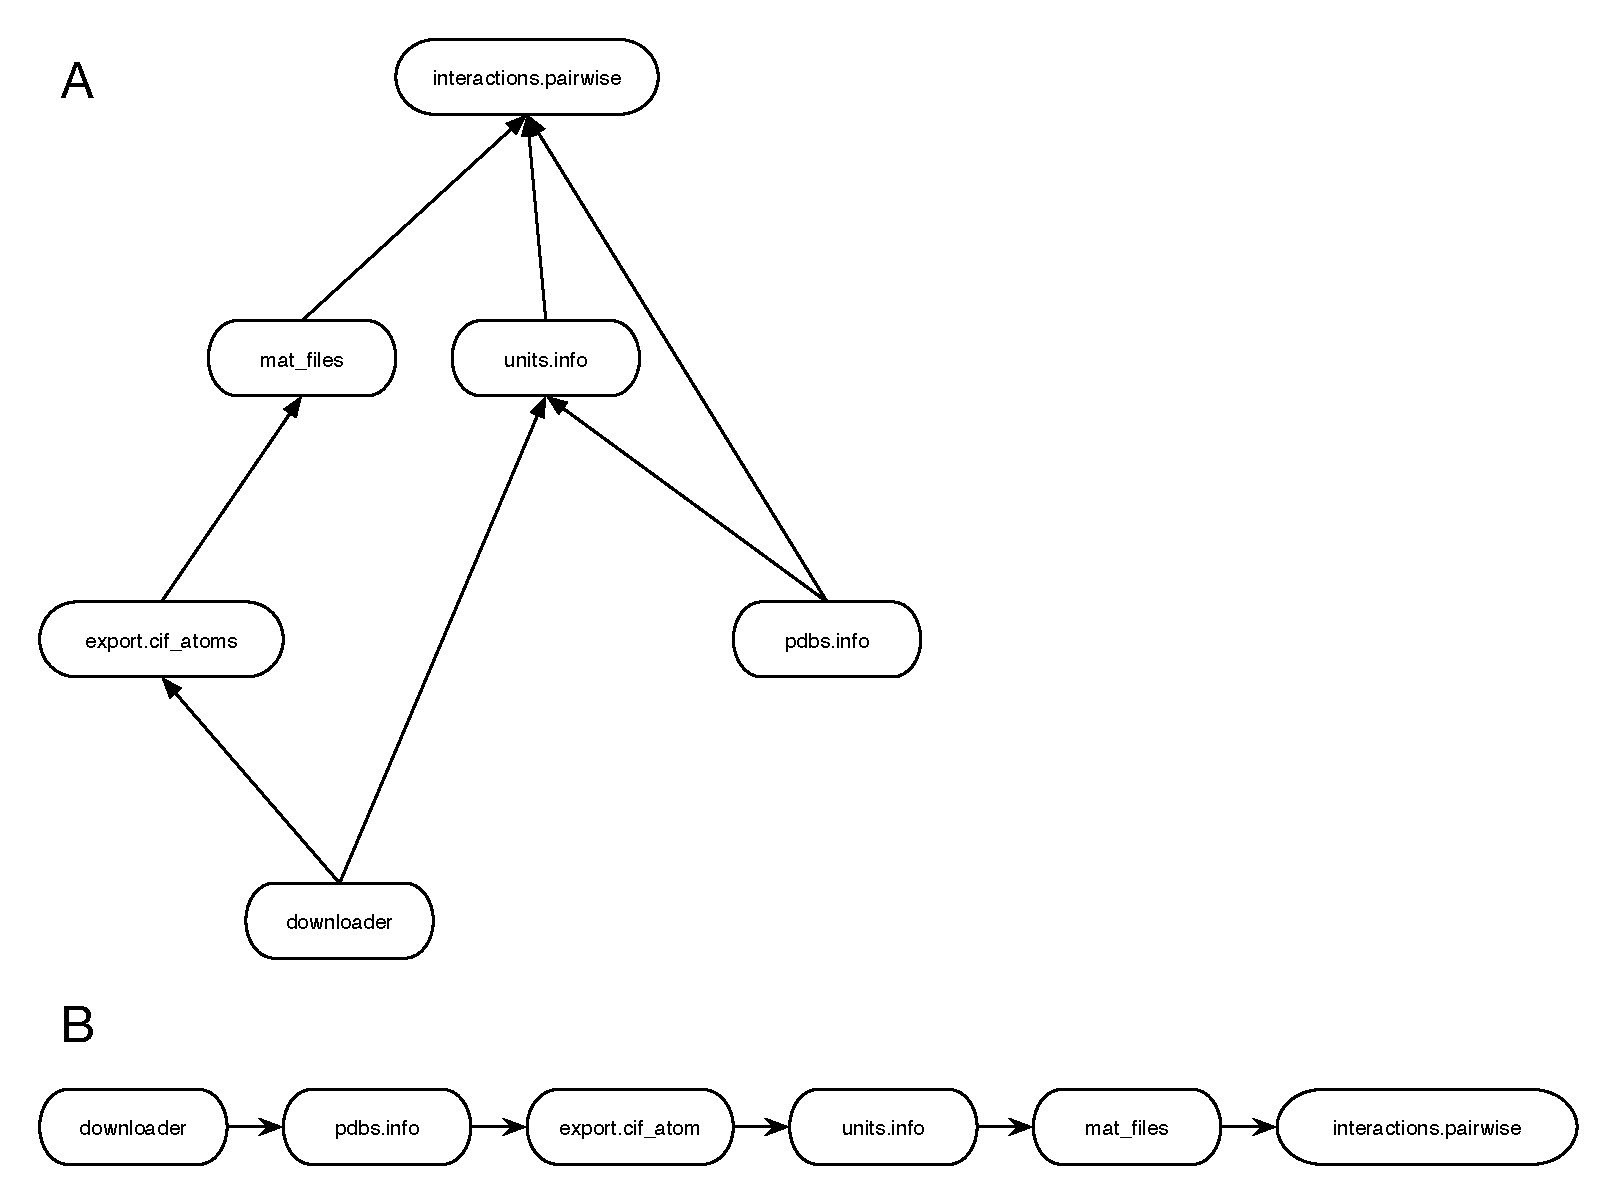
\includegraphics[width=\linewidth]{chapter-2/figs/deps}
  \caption{An example of an unsorted dependency graph (top) and a topological
    sorted dependency graph (bottom). Each stage is represented by an oval with
    the name of the stage in the oval. In this case the user has requested that
    the ``interactions.pairwise'' stage is run. This stage depends on two other
    stages, ``mat\_files'' and ``units.info'' as shown by the connections to those
    stages. Those stages have further dependencies. Shown in the bottom is the
    result of topological sorting the stages.}
\label{fig:stage-deps}
\end{figure}

With dependencies encoded in the pipeline, operators of the pipeline can request
the pipeline run a set of stages at once. In addition, part of the input to the
pipeline may optionally specify which dependencies do not need to be run. This
allows for the expression of complex requirements like, ``rerun all unit level
annotations except the distance and coordinate computation'. This is often
useful when testing out new parts or after fixing failed runs. When running all
structures, simply checking which input needs to be processed can take several
hours for some stages. When fixing a failed run or testing a new annotation, the
programmer will often already know which stages have been run. By instructing
the pipeline to run only those stages that are needed the overall run time can
be decreased.

With the previous version, to accomplish something similar to this it was
necessary to edit the code each time. I did this on several occasions and found
that it was very possible to forget that some parts were edited, since
computations could take hours, and in doing so left the code in a bad state for
the next weekly update. Because some parts were edited we did not run a complete
pipeline, leading to unexpected failures. This was then fixed by undoing the
edits that I previously made. Providing the capability to the pipeline operator
to what to run we avoid this problem entirely.

In addition, the main entry point now accepts either a list of PDB structures to
process or options to fetch the structures to run. The options and their usage
is explained in more detail in the ``Operation of the pipeline'' section. The
previous version always used all structures by default. While this is typically
the case, there are many situations where the operator wants to alter the
operation of the pipeline. For example, if one structure was not correctly
imported, only the failed structure should be rerun. By allowing the user to
select the structures specifically we make the pipeline easier to control.The
default mode of operation nonetheless remains. I have also added options to
allow selection of all structures that were available as of a specified date, or
prior to the current one. This has proven extremely useful when computing in old
releases during the update.

Operation of the the pipeline has been facilitated by implementing a single
entry point that takes as in input specifications for those parts parts to be
run and structures to be used. This ease of use also makes the pipeline more
reliable as it is no longer necessary to alter code to customize pipeline
operation.

\subsection{Making the pipeline robust to failures}

The pipeline will inevitably encounter errors during its operation. A robust
pipeline is one that gracefully fail. These errors can result from many sources.
The most obvious are mistakes in the code itself, for example, the pipeline may
have a bug in new code that causes it to attempts to for example, write invalid
quality data (a new feature). The second are errors introduced by external
resources. Part of our weekly update procedure is to fetch the list of all files
that are available as of the current date. This request to PDB can fail, because
all networks subject to intermittent failure. The final type of error is
mistakes in the input we are processing. For example, mmCIF files have certain
assumptions about their structure. In the past, some mmCIF files have not
respected their own assumptions leading to errors arising in the pipeline.I have
encountered all three types of errors and have worked to make the pipeline
robust in the face of these issues as discussed in the next paragraphs.

For the first set of errors, bugs in the code itself, I have added extensive
error handling code. The handling covers all aspects of the computing of and
saving of data to the database. Error handling identifies when errors occur and
alerts the user to the cause. Combined with extensive logging his aids in
debugging. The pipeline can cleanup, as required for validity, as well as
attempt to continue with other inputs. In addition, because the pipeline assumes
each input to a stage is independent and thus does not fail right away. This
leads the pipeline to attempting to compute data for all inputs to a stage prior
to failing. This provides a robustness against failures for specific inputs.

The next set of possible errors are those due to external resources. An example
of this type of work is fetching the quality report for a structure. PDB
provides quality data for all structures on their FTP site, which the pipeline
fetches for import. These requests can fail because of an unstable network.
However, these network errors are transient. The best way to handle network
errors is by identifying them as such and resubmitting the request.

I have modified the pipeline to retry requests to all external resources. Since
any request may fail due to network errors, the pipeline is now programmed to
always retry when a network error is encountered. It will retry up to the
specified number of attempts before failing. This allows for the pipeline to
deal with intermittent network failures, but not persistent failures. Longer
term issues such as a complete failure of the network will still cause the
pipeline to fail. However, this is acceptable since the pipeline could not
compute the required data. In addition, the requests can validate their
response. This helps with dealing in errors that happen when external sites
claim they sent data but the pipeline receives no data. For example, in the past
when querying PDB's services to attain the list of all files, PDB's response was
empty. This is not true as at the time about 2000 files were available, however
due to some error in their services we received a response stating there files
available.

The final type of issue, mistakes in the input data, does not have a simple
solution. Throughout the code, I have added checks to ensure the data is valid.
This allows confidence that the data being computed is correct. However, there
is no general purpose reusable way to always check that the mmCIF file is
formatted correctly. In addition we cannot simply retry computations as the data
will still be formatted incorrectly leading to the same errors. I dealt with the
issue mentioned above, a mmCIF violating its own design assumptions with
additions to the mmCIF reader to deal with this specific issue. I have added
extensive logging to the pipeline so that when this type of issues arises again
it will be flagged.

\subsection{Ease of extension}

The pipeline must be easy to extend. In order to make this possible I have
centralized all the essential logic of the pipeline into a few core classes that
can be inherited when creating a new stage. A class according to wikipedia is
"an extensible program-code-template for creating objects, providing initial
values for state (member variables) and implementations of behavior (member
functions or methods" \cite{Wiki2016}. Python, which the pipeline is mostly
written in, is an object-oriented language and users interested in working with
it are strongly recommended to study the language. The majority of the pipeline
is written using an intermediate or beginner level of python. None of the
advanced features, metaclasses for example, are used. I will attempt to explain
some fundamentals of python and object-oriented programming here.

Classes can ``inherit'' behaviors from other classes. This is commonly done
through ``inheritance'. Inheritance is a common feature of object oriented
programming where in there is a base class or parent which defines some
functionality. From there one or more classes ``inherit'' the functionality and
are called ``child'' classes. This relationship forms a hierarchy of classes. The
behavior of any class is defined by the code in the class and all parent
classes. The child class can then extend the parent class functionality by
adding new behaviors. In addition, the child may override the parent class
behaviors by providing it's own implementation of specific behaviors. The child
implementation of any behavior is always prefered over the parent behavior.

In the pipeline there is a parent class that defines the overall stage flow
shown in Figure~\ref{fig:stage-flow}. Users can add a  new stages, called the
``child'' class, which ``inherit'' from this parent class and receives all the
standard behaviors such as deleting failed imports and only recomputing when
needed. A user may decide that some stage should never delete data in the case
of a failed import. For example, our loop ids are meant to never change and
allowing automatic deletion may cause issues. Thus if we want to be safe the
class that implements the logic of importing loops overrides the deleting
behavior to do nothing except log an error.

Because classes inherit the essential functionality of the pipeline, new users will only have to
implement 1) the logic for querying the database to see if this structure has already been
processed and 2) the logic to create the data to store.
Operation of the pipeline
In this section, I discuss the RNA.BGSU.EDU pipeline at a high level, to familiarize readers with
its functionality, organization, operation and documentation. Salient details will be provided,and
complete references will be provided to direct readers to the relevant sections of the detailed
documentation. We begin with an overview of the structure of the code and of the application,
followed by configuration options, and end with directions for running the pipeline.

\section{Execution of the pipeline}

The pipeline is a Python and matlab application that is publically accessible at
\href{https://github.com/BGSU-RNA/RNA-3D-Hub-core}. Detailed documentation is
available for the python code at \href{http://rna-3d-hub-core.readthedocs.io/}.
Our relational database is MySQL and the schema is not currently public.

The application is organized into a series of directories, as shown in
Figure~\ref{fig:pipeline-organization}. This figure displays the key directories
and explains their contents.

\begin{figure}
  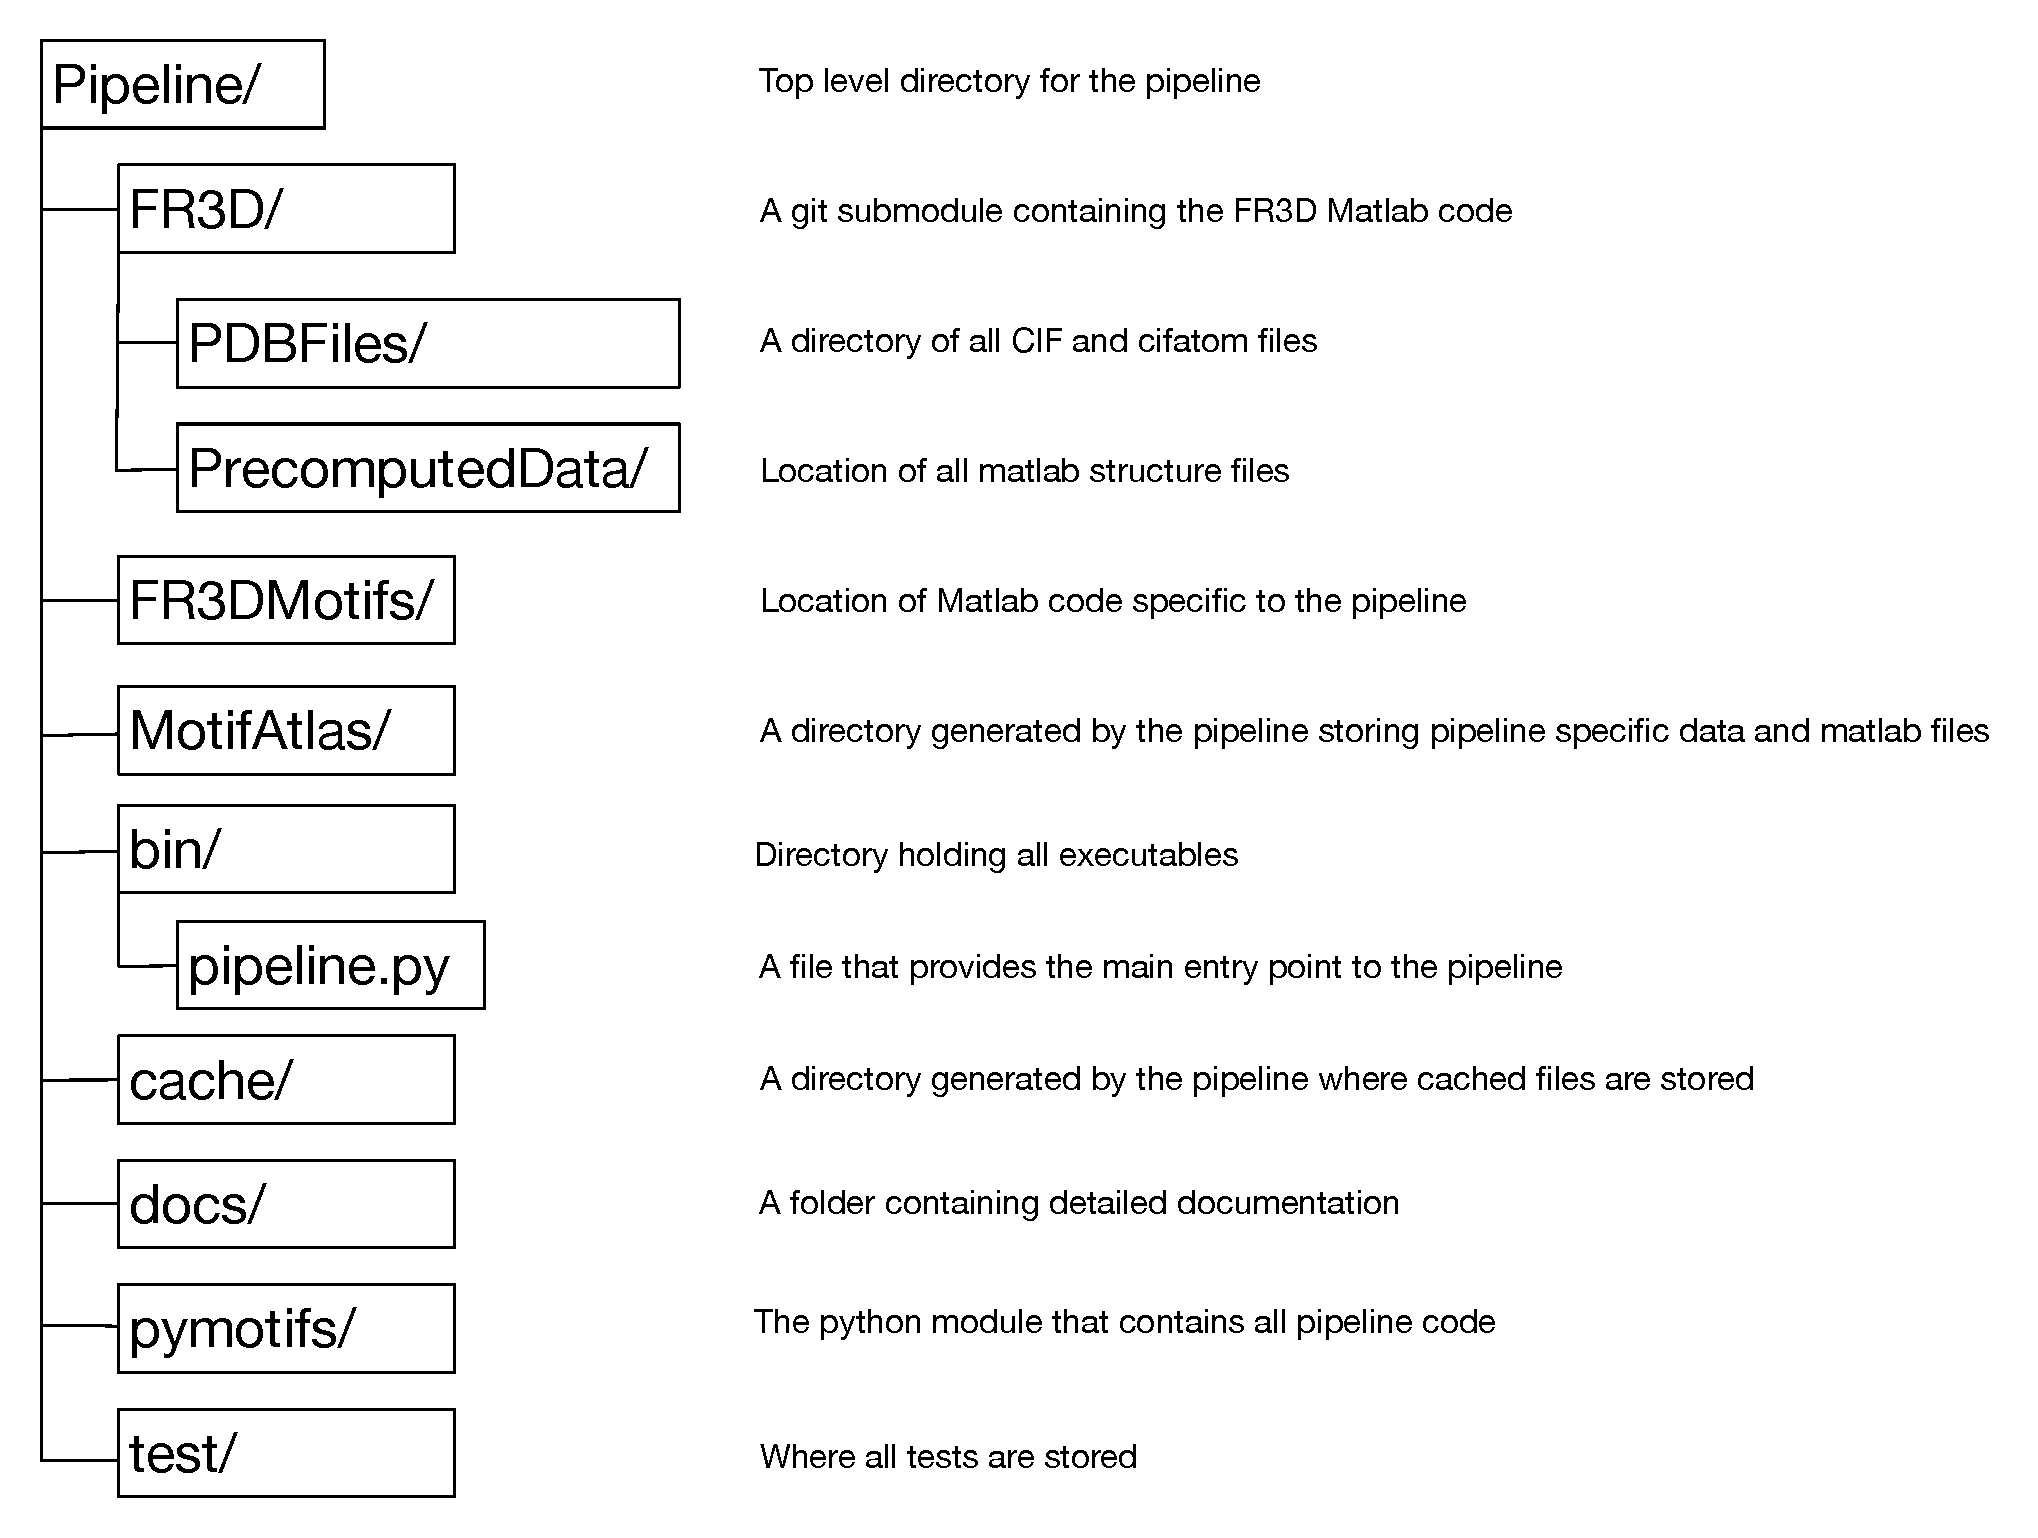
\includegraphics[width=\linewidth]{chapter-2/figs/directories}
\caption{Directory structure of the RNA BGSU pipeline. This figure shows the top
level and important directories in the pipeline. The directories are indicated
by ending with a ``/', while files do not end with a ``/'.}
\label{fig:pipeline-organization}
\end{figure}

\subsection{Configuring the pipeline}

Several important values, such as the database to use are configured in an
external file. The pipeline is configured through a JSON file that defaults to
``conf/motifatlas.json'. There are many possible configuration values, as
discussed in the detailed documentation. Table~\ref{tab:pipeline-config}
contains the key options. An example configuration file is included at
``conf/motifatlas.json.txt'' that can be modified to a simple working file. The
most important configuration value is the ``db.uri'' value which configures the
SQLAlchemy URI for the database connection. This specifies the database which to
connect to as well as the username and password. The user must be able to modify
the database, as well as add, delete and modify rows.

In addition, there are three file and directory paths which must be specified.
The first is the path to the matlab script that can execute matlab on the
command line. On linux systems this can be found using ``which matlab'' at the
command line and defaults to ``/usr/local/bin/matlab'. On OSX this will be in the
``bin/matlab'' directory below the matlab application. This means the default
location is ``/Applications/MATLAB\_R2013a.app/bin/matlab', for Matlab 2013a. The
second is where to write the loop export files. Part of the pipeline is an
export of all loops along with motif assignments. The file to write to must be
specified. Finally, the path to write interaction exports to must be specified
as well. Both the loop export an interaction export must be in a writeable
directory for the use the pipeline runs as.

Finally, the release\_mode section configures how the version numbers for motif
atlas, non- redundant and loops will be bumped. All releases follow the same
naming scheme of ``major.minor'. For example the NR release ``2.0'' has major
version ``2'' and minor ``0'. The minor can increments as much as needed and does
not influence the major version. When the major increments the minor is reset to
0. When the release\_mode is set to ``minor'' this will increment the minor part
of the version number, while ``major'' will cause the major to be bumped.
Generally, the release\_mode should be set to ``minor'. The only time ``major'
should be used is when there are large changes to the algorithm used for the
underlying algorithm.

\begin{table}[ht]
\begin{tabulary}{\linewidth}{LR}
\toprule
Variable & Purpose \\
\midrule

db.uri & SQLAlchemly uri string to specify the database to connect to \\

release\_mode.loops & A string, either ``major'' or ``minor'' to indicate
                        incrementing the major or minor version for loop releases \\

release\_mode.motifs & A string, either ``major'' or ``minor'' to indicate bumping
                        the major or minor version for motif releases \\

release\_mode.nr & A string, either ``major'' or ``minor'' to indicate bumping the
                   major or minor version for non- redundant releases \\

locations.mlab\_app & Path to matlab executable. \\

locations.interactions\_gz & Path to where the interactions export file is
                   written. \\

locations.loops\_gz & Path to where the loops export is written. \\

\bottomrule
\end{tabulary}
\caption{Main configuration options for the pipeline. All options show here must
  be provided.}
\label{tab:pipeline-config}
\end{table}

\subsection{Executing the pipeline}

The main entry point of the pipeline is the ``bin/pipeline.py'' python script. For
this discussion the script will be written as ``pipeline.py'. This script uses a
common ``subcommand'' ``options'' ``arguments'' design that will be familiar to anyone
who has used command line tools such as git. The top level command has a
``--help'' option which provides help information about the entire pipeline. In
addition, each subcommand also has a ``--help'' option to provide help information
about that command. Users should use this functionality extensively when
becoming familiar with the pipeline. In general a command to run the pipeline
looks like:

\begin{alltt}
pipeline.py [options] <subcommand> [options] [arguments]
\end{alltt}

Where $<>$ indicates a required value and $[]$ indicates an optional
value.

The pipeline provides several sets of functional facilities as shown in
Table~\ref{tab:pipeline-functionality}. This table shows each subcommand along
with the functionality it provides.

\begin{table}[ht]
\begin{tabular}{lr}
\toprule
Name & Functionality \\
\midrule
about & Get information about a stage \\
bootstrap & Populate the testing database \\
correct & A group of commands for correcting issues in the database \\
list & List the known stages and provide a breif overview \\
report & Create reports for external analysis \\
run & Run stage(s) \\
ss & Commands for importing 2D diagrams \\
transfer & Export/Import data from versions of this database \\
\bottomrule
\end{tabular}
\caption{Listing of all functionalities in the pipeline}
\label{tab:pipeline-functionality}
\end{table}

For the purposes of this section I will only discuss the import/export
functionality in the ``run'' subcommand. The main inputs to this command are the
stage to run and the structures to run it on. It takes a variety of options as
well. These options control the behavior of the pipeline. A summary of the
command is shown in Figure~\ref{fig:running-options}. Here we will discuss how
the options and arguments connect to our overall goals as well as how to achieve
some specific tasks.


\begin{figure}
\begin{alltt}
Usage: pipeline.py run [OPTIONS] NAME [IDS]...

  Run specific stages of the pipeline.

  'run' accepts as input the stage to run and a list of PDB ids to import
  and process. It determines the order of dependences and executes them in
  the correct order.

Options:
  --dry-run            Alter nothing while running
  --skip-dependencies  Skip stage(s)
  --skip-stage TEXT    Stage to skip
  --seed INTEGER       Set the random seed
  --recalculate STAGE  Recalculate data for the given stage(s)
  --all                Use all RNA containing PDBS
  --known              Use only downloaded files
  --after-date DATE    Get files posted after DATE (YYYY-MM-DD)
  --before-date DATE   Get files posted before DATE (YYYY-MM-DD)
  --exclude PDB        Excluded PDB(s)
  --ignore-time        Ignore time for rerunning
  -h, --help           Show this message and exit.
\end{alltt}
\caption{A summary of the options and arguments for the ``run'' subcommand.}
\label{fig:running-options}
\end{figure}

An important goal of our design has been to provide the user to ability to
choose the structures to process as well as the annotation data to compute. The
first was achieved by providing PDB ids as input. This input can be provided
manually when needed. It will process the files given and the user can input
them manually. As it is often the case that all available files, or all files
available by a date are wanted the pipeline accepts options which will determine
what files match that criteria. In addition, it is possible to then exclude
structures from that list using the given files.

The second goal, control over which data are computed, is done by putting the
stage to run as input to the pipeline. This provides the user precise control
over what is run. By default the pipeline will run all dependencies of the stage
as well the stage itself. This ensures that the required data are available for
the requested stage. When the user is sure that no dependencies need to be run,
I have added options to skip all dependencies ({\tt --skip-dependencies} ) or skip
specific stages ({\tt --skip-stage stage}).

Another goal is to avoid recomputing data already computed.where it is necessary
to over this default setting, the {\tt --recalculate stage} option can be used.
This option will force the pipeline to recompute all data for the given stage.
The {\tt .} stage name refers to the stage given so: {\tt pipeline.py run
--recalculate ``.'' --all units.info} will force a recompute for the units.info
stage, but not it's dependencies. To force all stages that are run to recompute,
the user can use the {\tt *} argument. For example {\tt pipeline.py run --all
--recalculate ``*'' units.info} will recompute all stages that are run for all
structures.

Examples that show how to use the described options and arguments will clarify
the usage. Below we list a series of tasks and the corresponding command
(displayed as {\tt monospaced font}).

\begin{description}
        \item [Run an update on all structures]
                {\tt pipeline.py run --all update}

        \item [Import pairwise interactions for 1FJG]
                {\tt pipeline.py run interactions.pairwise 1FJG}

        \item [Import all unit annotations for all structures]
                {\tt pipeline.py run --all units.loader}

        \item [Import all unit annotations for all structures skipping structure 2AW7]
                {\tt pipeline.py run --all --skip-pdb 2AW7 units.loader}

        \item [Create an NR group for 1FJG, 1J5E, 1S72]
                {\tt pipeline.py run nr.loader 1FJG 1J5E 1S72}

        \item [Compute all interaction annotations for all structures while skipping all dependencies]
                {\tt pipeline.py run --skip-dependencies --all interactions.loader}

        \item [Import loops in all structures]
                {\tt pipeline.py run --skip-stage loops.quality --all loops.loader}

                This command runs all loop level annotations, while skipping the loop quality stage,
                which is generally only needed before doing a motif atlas import, and simply is not
                needed importing loops, thus the reason it is skipped.

        \item [Recalculate all pairwise interactions]
                {\tt pipeline.py run --recalculate . --recalculate mat\_files interactions.pairwise}

                Note that for this command we have to recalculate all
                {\tt mat\_file}'' as well as the interaction import. This is
                because the {\tt mat\_files} stage controls the creation of the
                precomputed data that the matlab programs use. If we do not
                specify recomputing the mat files the process will simply
                reimport the already existing annotations.


        \item [Build a motif atlas using structures in the ``structures'' file]
                {\tt cat structures | xargs pipeline.py run motifs.loader}

                The structures file should contain only the ids to use, with one
                per line. The ``xargs'' command is required because the pipeline
                does not read from standard input and so xargs transforms the
                call to include the ids as part of the call. Note that there is
                a system dependent limit for the number of arguments allowed to
                a command. The limit is generally in the thousands.
\end{description}

\subsection{Testing the pipeline}

The pipeline is tested through two related methods. First, there is a script
that will run the pipeline on 70 structures to populate a test database. The
process of creating a database to work with is called ``bootstrapping''. The
structures to use are stored in ``pymotifs.constants.BOOTSTRAPPING'' and have been
chosen because they have caused crashes or errors in the past. In the future as
more problematic structures are found they should be added to the set of
structures used in testing.

The bootstrap script can be run using the command {\tt bin/pipeline.py bootstrap}.
Bootstrapping requires a special configuration file in conf/bootstrap.json. It
does not use the standard configuration file because it is important to have a
separate testing and development database. Otherwise it is possible to
accidentally overwrite or modify data that is required for tests. This can lead
to spurious test failures and waste developer time. Bootstrapping will run the
pipeline several times because one of the major parts of the pipeline is
computation of changes of groupings over time. By running it more than once on
different sets of structures we can test this important functionality.

The bootstrapping serves two purposes. The first is to populate a database the
test scripts can work with. The second is to provide a high level test of the
pipeline. By running the full pipeline on many structures we are increase the
chance of detecting blatant errors in the code. For example, bugs that prevent
the pipeline from being run will be caught here. Issues where a foreign key
constraint violation may appear here as well. This serves as a good initial
method to test the overall functionality of the pipeline and is recommended
before deploying a new stage.

The second way the pipeline is tested by ``unit testing'' components of the
pipeline. We test individual methods of classes using the py.test library. This
is a very traditional method of testing python applications. The tests are
stored in test/ and are organized into a hierarchy that parallels that of the
main program, making it simple to determine which module is being tested for
each test file. Test file names must end with ``\_test.py''. For example, the
tests for the units.info stage are in ``test/units/info\_test.py''.  There is very
extensive documentation on writing tests and readers are strongly encouraged to
read documentation on writing unit tests in python and using py.test. Examples
of such links are: 
\begin{itemize}
  \item \url{https://stackoverflow.com/questions/3371255/writing-unit-tests-in-python-how-do-i-start}
  \item \url{http://docs.pytest.org/en/latest/}
  \item \url{https://jeffknupp.com/blog/2013/12/09/improve-your-python-understanding-unit-testing/}
  \item \url{https://docs.python.org/2/library/unittest.html}.
\end{itemize}

Here we give a quick overview of testing in python, as well as information on
the parts that are unique to this pipeline.

In python, tests are often organized into classes. We use this approach
extensively in the tests. It is important to know that it is not needed, as
py.test will use simple functions as tests as well. Readers interested in that
approach should read py.test's documentation on this. We use classes because of
the organization advantages it provides. For test classes, if there is a ``setUp''
method that takes no arguments it is run prior to any tests. This method is used
to setup any data or objects that are needed for testing. As discussed below
this is used to setup stages for testing correctly. Each test method must start
with the string ``test\_'. Within them there should be an assertion about the
computed and expected value. Ideally tests are as simple as possible and contain
only 1 statement to compute the value to test, 1 statement to define the answer
and 1 statement to assert the computed value equals the expected value. This is
standard unit testing in python. The reader is encouraged to read more extensive
documentation and advice on this subject.

The test classes that test a stage in the pipeline must inherit from the
StageTest class from the test module. These classes should also have a
``loader\_class'' attribute which specifies the class of the stage to test. This
stage will be initialized in the StageTest's ``setUp'' method. The object will be
built using the configuration specified in ``conf/bootstrap.json''. As with
standard python tests this method is run prior to all test methods. Classes
which implement their own setUp method must have a call to the superclass's
setUp method. Without this the stage will not be initialized correctly.

Another useful functionality of the test suite is the ``skip\_without\_matlab''
annotation. This is to be used on any test that calls matlab. It allows the test
suite to run without crashing on machines that do not have matlab, or the python
to matlab connector, installed.

One useful extension to the testing methodology currently used is to automate
testing using a service like \href{https://travis-ci.org/}{Travis CI}. This
service reruns all tests whenever someone pushes code to the github repository.
Such testing has been implemented for the fr3d-python repository and can be seen
at \url{http://www.travis-ci.org/BGSU-RNA/fr3d-python}. Travis CI and related tools
are now standard in software development. This approach has not been used with
the pipeline for two reasons. First, setting up the database is a long and
complex procedure. The bootstrap script takes nearly half a day to run and
produces several gigabytes of data. Secondly, Travis CI and all services like it
do not have matlab installed as this is a commercial product. While the
skip\_without\_matlab annotation will ensure that other tests do not fail, it will
mean that key functionality that matlab provides will not be tested. This may
result in tests passing even though they are actually failing in an environment
with matlab. Thus we should not use the service as long as we continue to rely
on Matlab code.

It should be possible to deal with these issues by first, removing matlab from
the pipeline. Once all of FR3D's functionality is written in python the pipeline
will be testable with standard tools. Secondly, something will have to be done
to either decrease the number structures tested or make it quicker to load the
results of bootstrapping to the database. It may be possible to use a database
dump to rebuild the testing database, but that will pose problems with keeping
it up-to-date, but is worth exploring. Using a dump would mean the testing on
travis would not require the bootstrapping process, allowing for tests to be
completed quickly. Future developers should look into using tools like Travis CI
to improve the testing and reliability of the pipeline.
